\documentclass[a4paper,twoside]{article}

% The four publisher formatting files are used without modification.
\ifdefined\pdfinfoomitdate\pdfinfoomitdate=1\fi
\ifdefined\pdftrailerid\pdftrailerid{}\fi
\ifdefined\pdfsuppressptexinfo\pdfsuppressptexinfo=-1\fi
\usepackage{epsfig,subcaption,calc,amssymb,amstext,amsmath,amsthm,multicol}
\usepackage{pslatex,apalike,algorithm2e}
\usepackage[bottom]{footmisc}
\usepackage{graphicx,microtype,placeins,xcolor}
\definecolor{linkblue}{HTML}{3868D9}
\usepackage[unicode,colorlinks=true,linkcolor=linkblue,citecolor=linkblue,urlcolor=linkblue]{hyperref}
\let\mathematicalsup\sup
\usepackage{SCITEPRESS}
% SCITEPRESS reuses \sup for author-affiliation superscripts. Restore the
% mathematical operator in this anonymous mathematical manuscript.
\let\authorsup\sup
\let\sup\mathematicalsup
\hypersetup{
 pdftitle={When Can Finite-Context QELMs Replace Quantum Reservoir Memory?},
 pdfauthor={},pdfsubject={Anonymous editorial draft in ICAART 2027 format},
 pdfkeywords={Quantum Reservoir Computing, Quantum Extreme Learning Machines, Temporal Learning}
}
\graphicspath{{figures/}}
\newcommand{\doi}[1]{\href{https://doi.org/#1}{doi:\nolinkurl{#1}}}

% Keep full-width figures on separate pages without reducing their display size.
\setcounter{dbltopnumber}{1}

\begin{document}
\title{When Can Finite-Context QELMs Replace Quantum Reservoir Memory?}
% No author, affiliation, email, ORCID, date, or acknowledgements in review PDF.
\author{}
\keywords{Quantum Reservoir Computing, Quantum Extreme Learning Machines, Temporal Learning, Fading Memory, Finite Context.}
\abstract{We characterize when finite-window quantum extreme learning machines (QELMs)
can replace quantum reservoirs and when relevant information outside the window
prevents arbitrarily accurate emulation. The same information limit applies to
real-world temporal tasks whenever the required past information cannot be
recovered from the available input window.
We study reset-window QELMs, which reset for each prediction, and quantum
reservoir computers (QRCs), which carry a quantum state forward.
Under our assumptions, sufficiently expressive QELMs with growing windows
and exact expectations can approximate QRC outputs arbitrarily well precisely
when the missing past's influence fades uniformly. We quantify the unavoidable
window error and relate the required context to observable forgetting.
Persistent memory can prevent finite-window replacement. We construct a
simple quantum reservoir in which an old input can affect outputs
arbitrarily far into the future. Every fixed-window predictor therefore
faces an unavoidable worst-case error.
A QRC can solve the corresponding memory-recall task using exact
expectations; no reset-window QELM can match it uniformly over unbounded
delays, regardless of its capacity.
Analytical benchmarks and simulations examine three distinct limitations:
missing history, insufficient features, and finite measurements.
}
\onecolumn\maketitle\normalsize\setcounter{footnote}{0}\vfill

\section{INTRODUCTION}
\label{sec:introduction}

Whether a quantum extreme learning machine (QELM) can replace a quantum
reservoir computer (QRC) depends on more than model capacity: it depends on
access to the past. We establish when recent inputs contain enough
information to reproduce a reservoir's outputs, how much context is
required, and when persistent memory prevents replacement by any fixed
input window.

QRCs and QELMs offer two ways to process temporal data using quantum
features \cite{fujii2017harnessing,innocenti2023potential}. A QRC carries
its quantum state forward as new inputs arrive, allowing earlier events
to influence later outputs. The reset-window QELMs considered here instead
start afresh for each prediction and receive an explicit window of recent
inputs. Their memory therefore comes from the supplied data rather than a
state retained between predictions. Time-delayed QELMs demonstrate how
this approach can support time-series prediction without maintaining
quantum state throughout the input sequence \cite{kawanabe2026tdqelm}.
This makes the question of when a window can replace recurrence
practically relevant.

\begin{figure*}[t]
 \centering
 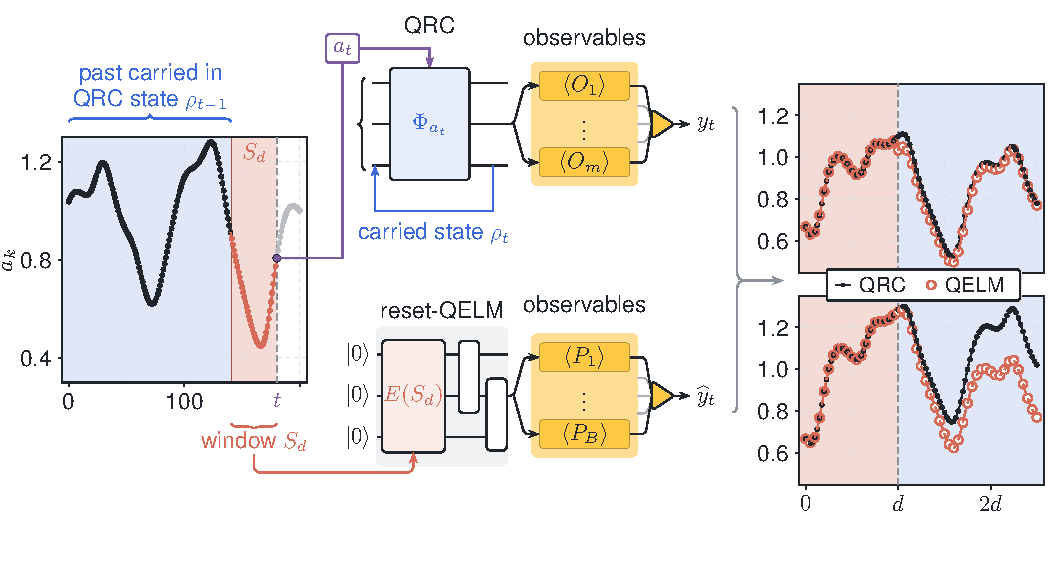
\includegraphics[width=\textwidth]{fig01_information_interface.pdf}
\caption{Two ways to provide memory: the QRC carries its quantum state
 forward, while the reset-QELM receives a window of recent inputs.
Right: an old input leaves the window at the dashed line. Above, its
influence has vanished by then, so the curves stay identical. Below, its influence
 becomes more visible and a gap remains. Orange denotes the QRC; blue
 denotes an ideal window prediction. These are schematic examples, not
 trained-model results: time advances while the window length stays fixed
 (Section~\ref{sec:models}). Here $E$ encodes the window, $O_j$ and $P_j$
 are measured observables, $m$ and $B$ count QRC outputs and QELM features,
 and $k$ indexes inputs while $t$ marks the current step.}
 \label{fig:information-interface}
\end{figure*}

The trade-off is between retaining history in a recurrent state and
supplying it explicitly through an input window. A QRC can preserve useful
information from much earlier inputs without replaying them, but its
dynamics must retain that information reliably. A reset-window QELM avoids
carrying quantum state between predictions and makes the available history
explicit, but expanding the window can require additional encoding and
processing resources. Neither approach is automatically more accurate or
more efficient: the appropriate choice depends on how much history the task
requires and the resources available to provide it.

Existing research provides complementary foundations for answering this
question. Quantum reservoir theory studies when dependence on the past
fades \cite{boyd1985fading,martinezpena2023finite}, while quantum
feature-model research establishes which functions sufficiently expressive
models can approximate \cite{goto2021universal}. We connect these
perspectives by separating two requirements: having the historical
information needed for an output, and having a representation capable of
using it.

The distinction is simple. Two input histories may have identical recent
inputs but different reservoir outputs because an earlier event still
matters. A window-only model cannot distinguish these histories, regardless
of its capacity. We quantify the resulting unavoidable error. Under our
stated assumptions and with exact expectation values, sufficiently
expressive QELMs can achieve arbitrarily accurate emulation as their windows
grow precisely when the omitted past's influence becomes uniformly
negligible across the allowed histories. We also relate the rate of
forgetting to the required context \cite{petreczky2026stability}. The
reservoir need not forget everything---only past information that can still
affect the chosen outputs matters.

Longer windows, however, do not always resolve the problem. We construct a
fixed two-qubit reservoir that performs temporal recall exactly using
expectation values. Over unbounded recall delays, every fixed-window
predictor faces the same positive worst-case error, regardless of its
capacity. This separates retained memory from finite context, rather than
quantum from classical computation.

Analytical benchmarks and simulations distinguish missing history from
limited features and finite measurements. The resulting guarantees concern
what a model can represent, not whether it can be trained efficiently or
implemented with fewer resources. Together, our results provide a practical
starting point for choosing between recurrent and window-based models:
first determine whether the available context contains the information the
task requires; then decide how best to represent and measure it.

\section{Quantum Reservoirs and Reset-Window Models}
\label{sec:models}

A QRC processes inputs one at a time. At discrete step $t$, input $a_t$
updates the previous state, and selected measurements provide the output
\cite{fujii2017harnessing,mujal2021opportunities}:
\[
 \rho_t=\Phi_{a_t}(\rho_{t-1}),
 \qquad y_t=\mathcal C(\rho_t).
\]
Here $\rho_t$ is the carried quantum state; the quantum channel $\Phi_{a_t}$
describes its physical evolution, including dissipation.
The fixed map $\mathcal C$ collects $m$ observable expectations
$\operatorname{Tr}(O_j\rho_t)$, $j=1,\ldots,m$: average measurement values,
shown as angle brackets in Figure~\ref{fig:information-interface}.
A trained linear readout can be included in $\mathcal C$ by absorbing its
fixed weights into the observables.

A reset-window QELM starts from the same quantum state for every prediction
and encodes the $d$ most recent inputs
\cite{innocenti2023potential,kawanabe2026tdqelm}.
For a history $h$ ending at $t$, with target output $y(h)=y_t$, its window is
\[
 S_d(h)=(a_{t-d+1},\ldots,a_t).
\]
The encoder $E(S_d(h))$ produces quantum features: observable expectations
of $P_j$, $j=1,\ldots,B$, including measurement checkpoints.
Thus $B$ counts measured expectations, not qubits.
A trained linear readout combines them. With exact expectations, the
complete prediction is
\[
 \widehat y_t=f(S_d(h)),
\]
where $f$ includes the quantum feature map and readout.

Identical windows therefore produce identical predictions for a
fixed model, even if earlier inputs differ.
With finitely sampled measurements, predictions can fluctuate, but their
probability distributions remain identical.
More qubits or features enrich the window function, but cannot recover
an earlier input that the window leaves unspecified.

For emulation we hold $\mathcal C$ fixed and target $y_t$, not the full state.
The emulation simulations use observable expectations directly; the separate
forecasting tests fit both readouts to external task targets.

Figure~\ref{fig:information-interface}'s output plots are schematic, not
fitted QELM predictions. The coral prediction is the conditional mean over two equally
likely old-input values with the same later inputs and known baseline.
Above, the old input is fully forgotten by window expiry, a special case
of fading memory. Below, later inputs gradually reveal retained information.
Sufficiency here concerns these example histories, not uniform accuracy
as the window length grows; Section~\ref{sec:criterion}
gives that criterion and the exact scalar error bound $D_d/2$. In the input
plot, $k$ indexes displayed steps and $t$ marks the current one.

\section{What a Finite Window Can Reproduce}
\label{sec:criterion}

A window can support accurate emulation only when histories with identical
recent inputs also produce nearly identical reservoir outputs. We quantify
the uncertainty left by the missing past, then establish when a sufficiently
expressive QELM can approach the best accuracy available from its window.

Consider histories with the same last $d$ inputs but potentially different
earlier inputs. Their largest output difference is
\begin{equation}
 D_d=\sup_{S_d(h)=S_d(h')}\|y(h)-y(h')\|.
 \label{eq:diameter}
\end{equation}
The supremum runs over all allowed histories. The norm is fixed and reduces
to absolute value for a scalar output. Thus $D_d$ measures how much the
output can vary when everything the window model receives is held fixed.

For a scalar output, each window is compatible with a range of reservoir
outputs. Predicting its midpoint minimizes the largest possible error:
any other prediction moves closer to one end but farther from the other.
If the range is $0.2$ to $0.8$, for example, predicting $0.5$ gives the
smallest worst-case error, $0.3$. Across all windows,
\begin{equation}
 \inf_f\sup_h |y(h)-f(S_d(h))|=\frac{D_d}{2},
 \label{eq:window-law}
\end{equation}
where $f$ ranges over all functions of the window. This limit applies
regardless of architecture or capacity. A longer window can reduce it by
distinguishing histories that a shorter window treats as identical. If
$D_d\to0$, arbitrarily small errors become possible in principle. If the
gap does not vanish, additional capacity cannot remove the error floor.

Approaching this limit with a QELM requires suitable dynamics and model
capacity. Assume a finite-dimensional reservoir, a compact input alphabet,
input-continuous quantum channels, and fixed observable outputs. Every
finite input continuation must be allowed after every admissible earlier
history. These conditions make the midpoint prediction continuous in
the window.

For each window length, let $\mathcal Q_d$ be a reset-QELM family that can
approximate every continuous window function uniformly as capacity grows,
using exact expectation values. Then, for scalar outputs,
\begin{equation}
 \inf_{f\in\mathcal Q_d}\sup_h
 |y(h)-f(S_d(h))|=\frac{D_d}{2}.
 \label{eq:qrc-qelm-equivalence}
\end{equation}
The family can approach the window's information limit arbitrarily closely.
This is an infimum: a particular finite model need not attain it exactly.

Consequently, under these assumptions, arbitrarily accurate QELM emulation
is possible precisely when $D_d\to0$ as the window grows. The omitted
past must become negligible uniformly across all allowed histories, not
only typical test examples. The same criterion holds for finite vector
outputs, although their unrestricted fixed-window optimum lies between
$D_d/2$ and $D_d$. Appendix~\ref{app:window-laws} provides the proofs and
shows that randomization cannot lower the scalar bound on worst-case
expected absolute error.

For inputs in $[0,1]$, repeated encoding and Bernstein approximation give
an explicit growing QELM construction
\cite{goto2021universal,yu2024nonasymptotic}. Its resource costs are discussed
next. This existence result neither guarantees efficient training nor
makes the fixed architectures in Section~\ref{sec:numerics} universal.
The replacement question is now one of memory: when do older inputs lose
their influence, and how much context makes their omission acceptable?

\section{DYNAMICAL ORIGINS OF OBSERVABLE MEMORY}
\label{sec:dynamics}

\subsection{Observable Forgetting}

An old input loses its influence if each new update shrinks differences
between earlier states.  Suppose every channel contracts trace distance
$D_{\rm tr}(\rho,\sigma)=\tfrac12\|\rho-\sigma\|_1$ by a uniform factor:
\begin{equation}
 D_{\rm tr}\!\left(\Phi_u(\rho),\Phi_u(\sigma)\right)
 \leq\eta D_{\rm tr}(\rho,\sigma),\qquad 0\leq\eta<1.
 \label{eq:incremental-channel}
\end{equation}
After $d$ common inputs, a scalar observable $O$ then obeys
\begin{equation}
 D_d\leq 2\|O\|_\infty\eta^d.
 \label{eq:contraction-bound}
\end{equation}
Old-state influence therefore falls exponentially, making finite context
sufficient for any fixed information-error tolerance.

The entire state need not forget.  Only differences that old inputs can
create and declared outputs can reveal matter.  Unreachable differences
cannot encode an input distinction; permanently invisible differences
cannot obstruct emulation.  Visibility must include future outputs, because
later inputs may reveal a currently hidden difference.

Restricting to the span of reachable differences and identifying those
indistinguishable under every future input gives the
\emph{reachable-observable quotient}.  Each channel induces a linear update
$A_u$ on this space.  Their joint spectral radius tests the long-term
damping over all input sequences:
\begin{equation}
 r_{\rm vis}
 =\lim_{d\to\infty}
 \sup_{u_1,\ldots,u_d}
 \|A_{u_d}\cdots A_{u_1}\|^{1/d}.
 \label{eq:visible-radius-definition}
\end{equation}
It measures the slowest asymptotic damping over allowed input sequences and
does not depend on the norm used.  The Appendix gives the quotient
construction and its norm properties
\cite{rota1960joint,jungers2009joint}.

\textit{Observable-memory theorem.}  For finite-dimensional QRCs with a
compact input alphabet, input-continuous channels, a fixed finite observable
output vector, and freely concatenable suffixes, the reachable-observable
joint spectral radius satisfies
\begin{equation}
 D_d\to0\quad\Longleftrightarrow\quad r_{\rm vis}<1,
 \qquad
 \lim_{d\to\infty}D_d^{1/d}=r_{\rm vis}.
 \label{eq:visible-memory-theorem}
\end{equation}
The missing past becomes uniformly negligible exactly when all relevant
state differences are uniformly damped.  The Appendix proves this by
comparing $D_d$ with the largest length-$d$ update product up to fixed
factors.  Individual-channel spectra do not suffice: a suffix can contain
arbitrary channel products.  Full-state contraction is unnecessary because
unreachable and permanently invisible directions have been removed.

This criterion also determines how much explicit context is needed.
For scalar output, let
\begin{equation}
 d_\varepsilon=\min\{d:D_d<2\varepsilon\}
 \label{eq:context-length}
\end{equation}
be the shortest window for which some unrestricted predictor has worst-case
error below $\varepsilon$.  When $0<r_{\rm vis}<1$,
\begin{equation}
 \lim_{\varepsilon\downarrow0}
 \frac{d_\varepsilon}{\log(1/\varepsilon)}
 =\frac{1}{-\log r_{\rm vis}}.
 \label{eq:window-complexity}
\end{equation}
Slowly fading observable memory therefore requires a long explicit context.
This law concerns the information requirement, not the feature or training
cost of a QELM.  Under full-state contraction,
$r_{\rm vis}\leq\eta<1$; the next construction realizes the opposite
boundary, $r_{\rm vis}=1$.

% Queue the resource figure for the experiments page without a late float gap.
\begin{figure*}[t]
 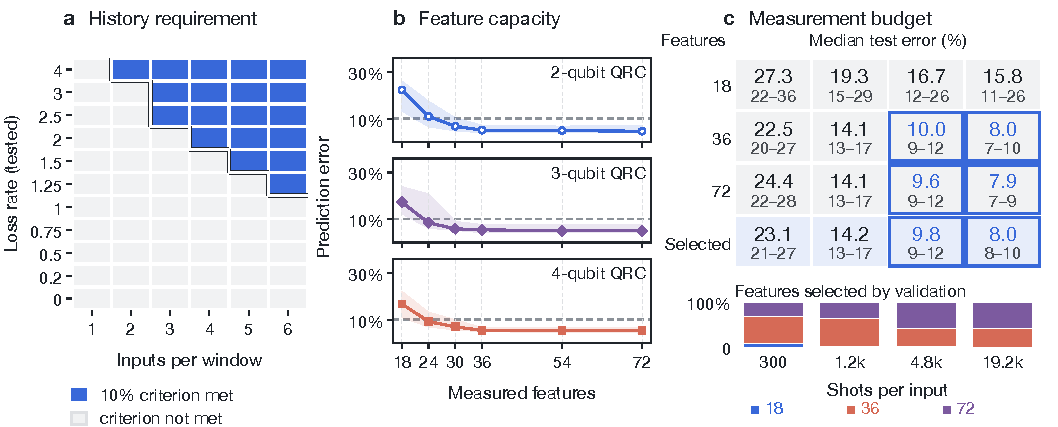
\includegraphics[width=\textwidth]{fig03_resource_diagnosis.pdf}
 \caption{Three resources address three limits.  Errors are NRMSE percentages;
 dashed lines mark $10\%=0.10$.  a,b Two- and three-qubit targets:
 a Old-history error versus scaled context $\gamma_T\Delta t\,d$.
 b Total QELM error versus features at $\gamma_T=4,d=6$, where history is
 sufficient. Curves show size-wise root medians; whiskers span the
 10th--90th root percentiles, describing variability rather than confidence
 intervals.
 c Validation-selected test error versus shots, with root medians and the
 selected policy's 10th--90th percentile whiskers. This post-confirmatory
 four-qubit follow-up repeats complete fitting and selection 16 times per root.}
 \label{fig:resource-diagnosis}
\end{figure*}

\subsection{Protected Memory}

Two qubits provide a write--protect--read example.  An old local pulse
changes the population of the antisymmetric singlet state.  Subsequent
symmetric drives and collective loss preserve it.  Pauli correlations
reveal the difference after the old input has left the window.  The singlet
projector is
\begin{equation}
 P_-=|\psi^-\rangle\!\langle\psi^-|
 =\frac{II-XX-YY-ZZ}{4},
 \label{eq:protected-singlet}
\end{equation}
so its expectation can be recovered from $XX$, $YY$, and $ZZ$ measurements.

Every update uses the same time-homogeneous input alphabet $a=(u,q)$.
Here $u$ controls the symmetric drive and the flag $q$ permits an
addressable pulse on the first qubit.  Two histories differ only in an old
flagged input; afterward they receive the same sequence from the freely
iterable $q=0$ subalphabet.  For that sequence, the population difference
is conserved.  The Appendix gives the pulse calculation and exact gap;
the full channel and control parameters appear in the Appendix.

More generally, suppose two reachable states differ by $\delta>0$ in the
expectation of an operator $P$, and a nonempty suffix subalphabet can be
iterated freely after both histories.  If
$\Phi_u^\dagger(P)=P$ for each symbol in that subalphabet, every such suffix
preserves the difference.  With the declared scalar output
$Y=\operatorname{Tr}(P\rho)$,
\begin{equation}
 D_d\geq\delta\qquad\text{for every finite }d.
 \label{eq:protected-mode}
\end{equation}
Equation~\eqref{eq:window-law} then forces worst-case absolute error of at
least $\delta/2$ for every finite-window emulator.  The singlet construction
supplies one process and one trajectory pair for every window length,
giving $r_{\rm vis}=1$ in Eq.~\eqref{eq:visible-memory-theorem}.

Matched controls distinguish protection from slow decay: local loss reduces
the gap, while asymmetric collective loss breaks exact conservation without
necessarily causing rapid erasure.  The storage mechanism is quantum; the
information bound applies to both quantum and classical stateless window
models.  When this obstruction is absent, emulation still needs sufficient
features and measurement precision.

\section{NUMERICAL EXPERIMENTS}
\label{sec:numerics}

\subsection{Models and Evaluation Protocol}

The phase-map QRCs have two, three, or four qubits, random $XX$ couplings,
transverse fields, input-dependent drives, and local loss $\gamma_T$.
Inputs use a uniform 33-point alphabet on $[0,1]$; outputs are single-site
Pauli expectations and same-axis two-site correlations.  A fixed six-qubit
reset-QELM encodes $d\leq6$ recent inputs, evolves under independent random
$XX$ couplings, and records Pauli features at nested times.  We vary $d$,
feature budget $B\in\{18,36,72\}$, and circuit shots per input $Q$.
This fixed emulator is not the theorem's growing universal family.
The Appendix specifies the dynamics and training parameters.

An independent realization block, or root, fixes the target, streams, and
feature map.  Training, validation, test, and diagnostic streams are
separate.  Training determines standardization; validation selects the ridge
readout.  The confirmatory two- and three-qubit cohort has 12 roots.
The denser loss--window map uses disjoint seeds; a prospectively frozen
four-qubit follow-up has 12 new roots.  Cohorts are never pooled.

A held-out common-suffix panel combines different old histories with
identical recent inputs.  Their mean squared output variation is the
old-history term; the squared distance from their mean to the window
prediction is the residual emulator error.  These add exactly to panel
MSE [Eq.~\eqref{eq:panel-decomposition}].  This distribution-dependent
diagnostic does not estimate worst-case $D_d$ or $r_{\rm vis}$ directly.

\begin{figure*}[t]
 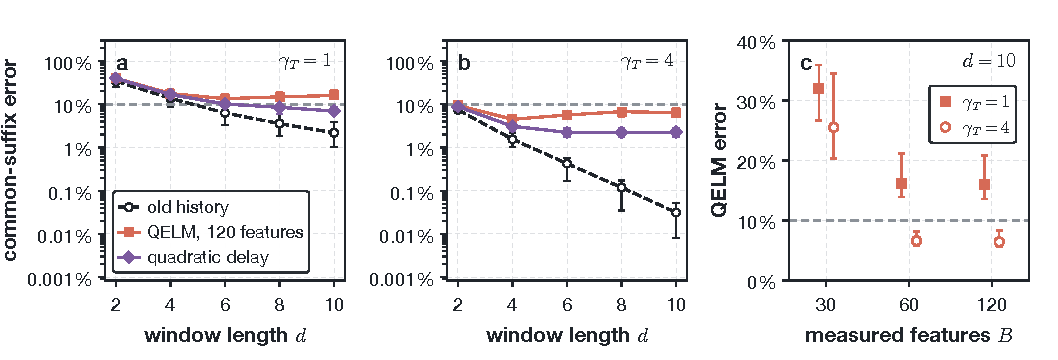
\includegraphics[width=\textwidth]{fig04_long_context_n5.pdf}
 \caption{Five-qubit targets and longer context.
 Separate prospective cohort: 12 new roots, a fixed ten-qubit reset-QELM,
 and all tested windows at $\gamma_T=1$ (a) and 4 (b).
 Common-suffix NRMSE compares the history floor, fixed $B=120$ QELM,
 and quadratic delay. Lines show root medians; whiskers span the
 10th--90th percentiles. The key applies to both panels; the gray dashed line marks 10\%.
 The larger register is an additional resource, not a matched-size advantage.}
 \label{fig:long-context}
\end{figure*}

Normalized RMSE (NRMSE) $0.10$ means 10\% of the target standard deviation.
A frontier cell succeeds when at least 10 of 12 roots meet this tolerance.
Confidence intervals use paired root-block bootstraps, not individual rows
or repeated measurements.

\subsection{History, Representation, and Measurement Limits}

The three questions are whether the window contains enough history, whether
features represent its output map, and whether shots resolve those features.
Under weak loss, old prefixes influence the output throughout the tested
window range.  Increasing loss shifts the measured frontier toward shorter
windows.  Across preregistered transition cells ($B=72$,
$\gamma_T\in\{2,4\}$), increasing $d=1\to6$ reduces held-out QELM NRMSE by a root median of $78.45\%$ (95\% CI
$[76.64,80.80]\%$), with the same direction in all 12 roots.

The dense maps test 11 loss rates and all integer windows from one to six:
198 cells across the two- and three-qubit cohort and the separately frozen
four-qubit follow-up.
Every rootwise local-loss decay fit has negative slope in both confirmatory
sizes.  The independent four-qubit cohort also has negative slopes and a
non-increasing frontier; every root reaches the inherited
$\gamma_T=4,d=6,B=72$ anchor.  Across all three sizes, no tested window is
history-sufficient through $\gamma_T=1$; the minimum falls to two by
$\gamma_T=4$.  The tested minimum history windows coincide across sizes, while
minimum successful feature budgets and emulation outcomes differ.
For each size at $\gamma_T=2,B=72$, $d=5$ meets the total-error root rule
but $d=6$ does not.
This is a tested loss--window crossover, not an asymptotic size law.

The primary $0.10$, 10-of-12 rule was preregistered.  A post hoc check uses
tolerances $0.08$, $0.10$, and $0.12$ with 9, 10, or 11 required roots.
Crossing cells change, but all 27 measured, right-censored
size--tolerance--rule frontiers remain non-increasing with loss.

On the fast-forgetting slice, limits appear in sequence.  At
$d=1,B=72$, all roots are history limited.  At $d=6,B=18$, the history
target is met but the fixed QELM is usually representation limited in the
operational sense defined in Section~\ref{sec:methods}. At
$d=6,B=36$, every root across all three sizes reaches the tolerance.
Figure~\ref{fig:resource-diagnosis}(b) shows the feature dependence for the
two- and three-qubit targets.

On the history-sufficient slice $\gamma_T=4,d=6$, increasing the QELM budget
from $B=18$ to 72 reduces common-suffix residual emulator NRMSE by a root median
of $67.26\%$ (95\% CI $[55.33,75.63]\%$), with the same direction in all 12
roots and both confirmatory sizes.  At $B=72$, all 24 confirmatory
root-by-size cases are emulated.  Features do not change the old-history term.

The exploratory post-confirmatory shot study independently samples training,
validation, and test features; target outputs remain exact expectations.
Validation-selected test NRMSE falls from
$0.231$ at 300 shots per input to $0.0800$ at 19,200 shots, a $65.20\%$
reduction (95\% CI $[64.04,66.47]\%$), positive in all 12 roots.  Validation
selects $B=36$ most often at low shot counts and $B=72$ at high shot counts.
Extra features help when the measurement budget resolves them
[Figure~\ref{fig:resource-diagnosis}(c)]
\cite{hu2023sampling,ahmed2025finite}.

Linear delay, quadratic delay, and dimension-matched random-tanh controls use
the same windows and splits as the QELM.  Quadratic delay is the strongest
classical control in all 24 fast-forgetting confirmatory cases and outperforms
the $B=72$ QELM in every root. This is a resource diagnosis,
not quantum advantage.

With five-qubit targets and a ten-qubit reset-QELM
(Figure~\ref{fig:long-context}), increasing $d=2\to10$ reduces history NRMSE
by root medians of $93.55\%$ at $\gamma_T=1$ and $99.63\%$ at
$\gamma_T=4$, positive in all 12 roots at each loss.
At $\gamma_T=1$, windows 6, 8, and 10 meet the history rule but no tested
QELM budget meets the total-error rule. At $\gamma_T=4$, every window meets
the history rule; $B=60$ reaches the total-error target in all 12 roots
only from $d=4$ onward. Quadratic delay beats the fixed $B=120$ QELM in
118 of 120 streaming root--condition comparisons.

\FloatBarrier
\section{DISCUSSION AND CONCLUSIONS}
\label{sec:summary}

Finite-window emulation is limited by the history a model can access, not
by model capacity alone. Under our assumptions, sufficiently expressive
reset-window QELMs with exact expectations can approximate QRC outputs
arbitrarily well as their windows grow precisely when the influence of
the omitted past fades uniformly. We quantify the unavoidable error
caused by missing history and relate the context needed for a desired
accuracy to the rate of observable forgetting.

Conversely, our two-qubit construction preserves an old input's effect
on later outputs over arbitrarily long delays. Every fixed-window
predictor then faces a positive worst-case error floor that neither
additional features nor a longer finite window can remove. This
establishes a separation between carried memory and finite context,
rather than between quantum and classical computation. The guarantees
concern representability, not efficient learning or resource savings.

Analytical benchmarks and simulations distinguish three limitations:
missing history, insufficient features, and finite measurements. Their
practical message is to establish how much history the desired outputs
require before tuning how that history is represented and measured.
Missing information requires longer context or retained state;
increasing feature capacity alone cannot resolve it.

Together, these results provide a principled basis for designing and
comparing quantum temporal models. They identify when explicit context
can replace reservoir memory and when persistent observable information
prevents that replacement, making access to the past---not only the
richness of its representation---a central consideration in architecture
selection and resource allocation.

\bibliographystyle{apalike}
{\small\microtypesetup{expansion=false}\bibliography{references}}
% The publisher requires an unnumbered appendix after the references,
% continuing on the same page, within the one submitted paper.
\section*{APPENDIX}
\setcounter{subsection}{0}
\renewcommand{\thesubsection}{\Alph{subsection}}
\label{app:proofs}

\subsection{Optimal Window Error}
\label{app:window-laws}

\emph{The best prediction for a fixed window.} Let $\mathcal R$ be the
closure of states reachable before a window $s=(a_1,\ldots,a_d)$, and
write $\Phi_s=\Phi_{a_d}\cdots\Phi_{a_1}$. Under
Section~\ref{sec:criterion}'s assumptions, $\mathcal R$ is compact and
independent of $s$. For scalar output, define
\[
 y_-(s)=\min_{\rho\in\mathcal R}\mathcal C\Phi_s(\rho),\quad
 y_+(s)=\max_{\rho\in\mathcal R}\mathcal C\Phi_s(\rho).
\]
Any prediction must be at least half this range away from one endpoint.
The midpoint $m_d(s)=[y_-(s)+y_+(s)]/2$ achieves this bound. Taking the
worst case over windows gives the optimal error $D_d/2$. Using the
reachable closure does not change this supremum.

\emph{Why QELMs can approach the optimum.} Continuity of the channels
on the compact window--state domain makes $y_-$, $y_+$, and $m_d$
continuous. Uniform QELM density therefore supplies a predictor within
any $\varepsilon>0$ of $m_d$, with total error at most
$D_d/2+\varepsilon$. This proves an infimum; a finite model need not
attain it exactly.

For vector outputs, the triangle inequality still gives the lower bound
$D_d/2$. Replaying the window from any fixed reachable state gives a
continuous predictor with error at most $D_d$. Approximating this replay
function proves that arbitrarily accurate emulation is possible exactly
when $D_d\to0$.

\emph{Randomness cannot recover missing history.} Two histories with
the same window induce the same prediction distribution. For their
scalar outputs $y_0,y_1$,
\[
 |y_1-y_0|\leq\mathbb E|y_0-\widehat y|+\mathbb E|y_1-\widehat y|.
\]
At least one expected absolute error is therefore at least half the gap.
Randomized predictions cannot lower the worst-case information floor.

\subsection{Observable Memory and Required Context}
\label{app:observable-proof}

\emph{Keep only differences that can affect an output.} Let $\Delta$
be the compact set of reachable state differences, including limits,
and let $V=\operatorname{span}_{\mathbb R}\Delta$. A difference is
irrelevant if no future input sequence can reveal it. Remove these
differences by defining
\[
 \mathcal N=\{v\in V:\mathcal C\Phi_w(v)=0\text{ for every finite word }w\}.
\]
The empty word is included. On $W=V/\mathcal N$, the induced update
and output maps are $A_a[v]=[\Phi_a(v)]$ and
$\overline{\mathcal C}[v]=\mathcal C(v)$. This is the
reachable--observable reduction used in
Section~\ref{sec:observable-forgetting}, specializing
\cite[Theorem~III.1]{petreczky2026stability}.

\emph{Measure memory by its possible future effect.} On $W$, define
\[
 \|x\|_{\rm obs}=\sup_w\|\overline{\mathcal C}A_wx\|.
\]
The invariant reachable set makes this finite, and removing $\mathcal N$
makes it a norm. Let $c_d=\sup_{|s|=d}\|A_s\|_{\rm obs}$, using the
induced operator norm.

Appending common inputs preserves reachability, so
$\Phi_w(\Delta)\subseteq\Delta$ for every word $w$.
Absorbing the first $\ell$ inputs of a length-$(d+\ell)$ word into
its starting difference therefore gives $D_{d+\ell}\leq D_d$.
For $v\in\Delta$, $|s|=d$, and any future word $w$ of length $\ell$,
\[
 \|\overline{\mathcal C}A_wA_s[v]\|\leq D_{d+\ell}\leq D_d.
\]
Taking suprema gives the upper bound $D_d$. The empty future word
recovers $\sup_{v\in\Delta,\,|s|=d}\|\overline{\mathcal C}A_s[v]\|=D_d$,
establishing equality.

The convex hull of the reachable differences
in $W$ contains a norm ball and is bounded. Thus constants
$\kappa_-,\kappa_+>0$, independent of $d$, satisfy
\[
 \kappa_-c_d\leq D_d\leq\kappa_+c_d.
\]
This comparison connects observable output gaps to the size of products
of the reduced updates.

\emph{Decay rate and window length.} The product norms satisfy
$c_{d+\ell}\leq c_dc_\ell$. Hence $D_d\to0$ implies $c_{d_0}<1$ for
some $d_0$, which forces exponential decay. Conversely, $r_{\rm vis}<1$
gives exponential decay of $c_d$ and therefore of $D_d$. Taking $d$th
roots in the comparison above yields
\[
 \lim_{d\to\infty}D_d^{1/d}=r_{\rm vis}.
\]
For $0<r_{\rm vis}<1$, bounding $D_d$ between $r_-^d$ and $r_+^d$ for
sufficiently large $d$, where $0<r_-<r_{\rm vis}<r_+<1$, and solving
$D_d<2\varepsilon$ gives
\[
 \lim_{\varepsilon\downarrow0}\frac{d_\varepsilon}{\log(1/\varepsilon)}
 =\frac{1}{-\log r_{\rm vis}}.
\]
If $W=\{0\}$, set $D_d=r_{\rm vis}=0$. The argument assumes freely
concatenable inputs; constrained input grammars require a separate
analysis.

\subsection{An Explicit QELM Construction}
\label{app:bernstein-resources}

\emph{Assumptions.} For a quantitative bound, take inputs in $[0,1]$,
scalar output $y=\operatorname{Tr}(O\rho)$, and $M=\|O\|_\infty$.
In addition to the assumptions above, suppose
\begin{equation}
 D_{\rm tr}(\Phi_a(\rho),\Phi_{a'}(\sigma))
 \leq\eta D_{\rm tr}(\rho,\sigma)+L_{\rm in}|a-a'|,
 \label{eq:incremental-lipschitz}
\end{equation}
with $0\leq\eta<1$. This is stronger than observable forgetting: it
requires uniform state contraction and Lipschitz dependence on the input.

\emph{Encode, measure, and average.} Encode each input $a_i$ in $r$
copies of $\sqrt{1-a_i}|0\rangle+\sqrt{a_i}|1\rangle$. Measuring each
block gives independent counts $K_i\sim\operatorname{Binomial}(r,a_i)$.
Assign the linear-readout coefficient $m_d(k_1/r,\ldots,k_d/r)$ to
count outcome $(k_1,\ldots,k_d)$. The expected prediction is the
Bernstein approximation
\[
 f_r(s)=\mathbb E\bigl[m_d(K_1/r,\ldots,K_d/r)\bigr].
\]
The midpoint inherits the input sensitivity bound
\[
 |m_d(s)-m_d(s')|
 \leq2ML_{\rm in}\sum_{i=1}^d\eta^{d-i}|a_i-a_i'|.
\]
Together with $\mathbb E|K_i/r-a_i|\leq1/(2\sqrt r)$, this bounds
the representation error. Averaging $Q$ independent readouts gives
$\widehat f_r$. Since each readout lies in $[-M,M]$, Hoeffding's
inequality~\cite{hoeffding1963probability} bounds its sampling error.
For each fixed history and $0<\zeta<1$, with probability at least
$1-\zeta$,
\begin{equation}
 |y(h)-\widehat f_r(S_d(h))|
 \leq D_d/2+\varepsilon_{\rm rep}+\varepsilon_{\rm shot},
 \label{eq:midpoint-resource-bound}
\end{equation}
where
\[
 \varepsilon_{\rm rep}=\frac{ML_{\rm in}(1-\eta^d)}{(1-\eta)\sqrt r},\quad
 \varepsilon_{\rm shot}=M\sqrt{\frac{2\log(2/\zeta)}{Q}}.
\]
With exact expectations, omit $\varepsilon_{\rm shot}$ and the bound
holds uniformly over histories. Contraction also gives
$D_d/2\leq M\eta^d$. The finite-shot guarantee is pointwise, not
simultaneous over all histories.

The construction uses $rd$ qubits and up to $(r+1)^d$ midpoint
coefficients. Computing these coefficients requires reachable-output
extrema and is not included in the resource count. This establishes
representability, not an efficient training procedure.

\emph{Analytical checks.} For the one-qubit channel in
Section~\ref{sec:sharpness}, the compatible populations have width
$D_d=\eta^d$ and midpoint
\[
 m_d(s)=\frac{\eta^d}{2}+(1-\eta)\sum_{i=1}^d\eta^{d-i}g(a_i).
\]
Thus any predictor $f$ has worst-case error
$\eta^d/2+\|f-m_d\|_\infty$. For $g(a)=a^2$, replacing $g(K_i/r)$ by
$K_i(K_i-1)/[r(r-1)]$ gives an unbiased readout for every $r\geq2$,
attaining the information floor exactly. For
$g(a)=(e^{2a}-1)/(e^2-1)$, the midpoint coefficients give a nonnegative
Bernstein bias. Additivity reduces the worst-case calculation to a
one-dimensional maximization of that bias. These checks use analytical
readouts and binomial expectations, not training.

\subsection{Protected Memory}
\label{app:protected-calibration}

\subsubsection{The Persistent Error Floor}
\label{app:protected-pulse}

Starting from $|00\rangle$, a first-qubit pulse writes singlet population
\[
 \delta=|\langle\psi^-|R_x^{(1)}(\theta)|00\rangle|^2
 =\tfrac12\sin^2(\theta/2).
\]
Without the pulse, this population is zero. Symmetric evolution with
collective loss preserves both populations during any unpulsed
continuation. The output gap therefore remains $\delta$ after arbitrarily
many shared inputs, giving $D_d\geq\delta$ and worst-case window error
at least $\delta/2$ for every finite $d$. A one-radian pulse gives
$\delta\approx0.1149$ and an error floor of approximately $0.0575$.
Conservation is needed only along these common continuations, not for
every possible input sequence.

\subsubsection{Dynamics and Controls}
\label{app:protected-implementation}

The numerical check uses
\[
 \begin{gathered}
 H(u)=JX_1X_2+0.37(Z_1+Z_2)+0.64u(X_1+X_2),\\
 L_c=\sqrt{0.8}(\sigma_1^-+\sigma_2^-),\qquad\Delta t=0.2.
 \end{gathered}
\]
Here $\sigma_i^-=|0\rangle\langle1|_i$ is the lowering operator.
Twelve independent realizations sample $J\in[-1,1]$ and 80-input
continuations with $u\in[0,1]$ after the optional pulse. Checks verify
the pulse value and singlet conservation. Matched local amplitude
damping reduces the median 80-step gap to $1.57\times10^{-5}$.
Relative collective-jump asymmetries of $0.02$, $0.05$, $0.10$, and
$0.20$ break exact conservation but need not erase the gap rapidly.
These controls distinguish protected memory from slow forgetting.

\subsection{Numerical Evaluation}
\label{sec:methods}

\subsubsection{The Common-Suffix Diagnostic}
\label{app:common-suffix-diagnostic}

Let $y_{sk}\in\mathbb R^m$ be the output for suffix $s$ and prefix branch
$k$, $\bar y_s$ its branch mean, and $\widehat y_s$ their shared prediction.
Here $\mathbb E_{s,k}$ and $\mathbb E_s$ are equal-weight empirical averages
over suffix--branch pairs and suffixes, and $\|\cdot\|_2$ is the Euclidean norm:
\begin{equation}
 \begin{aligned}
 &\frac1m\mathbb E_{s,k}\|y_{sk}-\widehat y_s\|_2^2\\
 &\quad=\frac1m\mathbb E_{s,k}\|y_{sk}-\bar y_s\|_2^2\\
 &\qquad+\frac1m\mathbb E_s\|\bar y_s-\widehat y_s\|_2^2 .
 \end{aligned}
 \label{eq:panel-decomposition}
\end{equation}
The vanished within-suffix cross term splits total squared error into
old-history and residual emulator contributions. Residual error includes
feature approximation, finite-data estimation, ridge regularization, and
suffix-mean sampling variability. It is not an isolated feature-approximation error.

With $n_{\rm pre}$ conditionally independent prefix branches, the history
numerator averages $(n_{\rm pre}-1)/n_{\rm pre}$ times population conditional
variance. The registered $n_{\rm pre}=4$ gives correction $4/3$, preserving
every emulated or representation-limited classification and all reported
window and feature effects. Equation~\eqref{eq:panel-decomposition} is exact
for uncorrected terms. Neither it nor the correction estimates $D_d$ or $r_{\rm vis}$.

\subsubsection{Models and Evaluation Protocol}

Targets (subscript $T$) have $N_T\in\{2,3,4\}$ qubits and local-loss rate
$\gamma_T$. Each fixed input $a$ drives
\begin{align}
 H_T(a)&=\sum_{i<j}J_{ij}X_iX_j+0.5\sum_i Z_i+a\sum_iX_i,\nonumber\\
 \dot\rho&=-i[H_T(a),\rho]+\gamma_T\sum_i\mathcal D[\sigma_i^-]\rho,
 \label{eq:target-qrc-model}
\end{align}
Here $\dot\rho=d\rho/d\tau$ uses physical time $\tau$, while $t$ indexes
discrete inputs. The dissipator is
$\mathcal D[L]\rho=L\rho L^\dagger-\tfrac12\{L^\dagger L,\rho\}$;
$\dagger$, $[\cdot,\cdot]$, and $\{\cdot,\cdot\}$ denote Hermitian adjoint,
commutator, and anticommutator. Couplings are uniform on $[-1,1]$,
$\Delta t=0.5$, and inputs use a uniform 33-point alphabet on $[0,1]$.
Single-site and same-axis two-site Pauli expectations give
9, 18, and 30 outputs, respectively.

The fixed six-qubit QELM resets and encodes the newest $d\leq6$ inputs as
$\sqrt{1-a}|0\rangle+\sqrt a|1\rangle$, leaving unused qubits in $|0\rangle$.
Independent uniform $[-1,1]$ $XX$ couplings and transverse field $0.5$
evolve the state for $\tau=0.5$ without dissipation.
Single-site $X,Y,Z$ expectations at one, two, or four
nested checkpoints give $B\in\{18,36,72\}$ observable--checkpoint features.

\emph{Cohorts and held-out data.} A root fixes target parameters, streams, and feature seeds.
The confirmatory cohort uses $N_T\in\{2,3\}$,
$\gamma_T\in\{0,0.2,0.5,1,2,4\}$, and $d\in\{1,2,4,6\}$.
The dense map adds $d=3,5$ and rates $0.75,1.25,1.5,2.5,3$ with
12 roots and 108 seeds disjoint from the original experiment.
The prospectively frozen four-qubit follow-up, designed after map inspection,
uses 12 new roots, 96 disjoint seeds, and otherwise unchanged settings.
Registered checks test negative
history decay, a non-increasing minimum-window frontier, and the
$\gamma_T=4,d=6,B=72$ anchor. Sizes are never pooled.

Training, validation, test, and suffix streams are independent. Streaming
splits start in $|0\cdots0\rangle$ with 128 washout steps before 480 training,
160 validation, or 320 test rows. Panels pair 32 length-six suffixes with
four independently burned-in prefixes each; shorter windows are nested tails.
Newest symbols are sampled without replacement from the alphabet, older
coordinates independently. Roots and cohorts have disjoint seed namespaces.

\emph{Fitting and decision rules.} Training alone standardizes features.
Validation selects the affine ridge penalty
\[
 \begin{aligned}
 \lambda\in\{&0,10^{-10},10^{-8},10^{-6},10^{-4},10^{-2},\\
             &1,10^2,10^4,10^6,\infty\},
 \end{aligned}
\]
then training and validation data refit the readout. Finite penalties use economy
singular-value decomposition with relative resolved-subspace cutoff $10^{-6}$;
$\lambda=\infty$ gives intercept-only prediction.

Linear delay, quadratic delay, dimension-matched random-tanh, intercept-only,
and reset--replay share windows and splits. Replay applies the last $d$ target
channels to a fixed state, refitting (retrained) or retaining (compiled) the
affine readout. Each cell selects its best nonconstant classical control.

The preregistered NRMSE tolerance $0.10$ is 10\% of the target standard
deviation. History or emulation passes if its error is at most $0.10$ in
at least 10 of 12 roots (one-sided probability $0.0193$ under fair nonzero
signs). Roots are independent units; rows, observables, suffixes, and shot
replicates are not. Confidence intervals use 20,000 paired root-block bootstraps.

After excluding variances below $10^{-8}$, diagnosis checks history-floor
failure, total-QELM success, then replay success. Representation limited
means history passes, the fitted QELM fails, and replay succeeds, not that
the best approximation using QELM features fails.

The $0.10$, 10-of-12 frontier predates dense-map inspection. Post hoc
sensitivity checks reuse simulations at tolerances $0.08$, $0.10$, $0.12$
and 9, 10, or 11 required roots.

\subsubsection{Finite-Shot Extension}

The exploratory post-confirmatory study uses 12 four-qubit local-loss targets,
$\gamma_T=4$, $d=6$, and $Q\in\{300,1200,4800,19200\}$ shots per input.
Snapshots and global-Pauli settings receive equal integer shares.
Joint multinomial bit-string draws give compatible single-site expectations.
Each of 16 replicates independently resamples training, validation, and test
features and repeats fitting. Validation selects $\lambda$ for each $B$,
then $B$, without test targets. Exact targets isolate emulator sampling.
Section~\ref{sec:numerics}'s intermediate-feature study uses exact expectations.

\subsubsection{Long-Context Extension}

The prospective cohort uses 12 new roots, $N_T=5$ (45 outputs),
$\gamma_T\in\{1,4\}$, and $d\in\{2,4,6,8,10\}$.
A fixed ten-qubit QELM encodes one input per qubit; nested checkpoints
give $B\in\{30,60,120\}$. Panels use 32 length-ten suffixes with four
prefixes each; other settings are inherited. Freezing follows two duplicate
development runs and dense-backend checks. All cells remain. Paired history
contrasts use 10,000 root-block bootstrap draws; the QELM--quadratic
comparison fixes $B=120$ before test evaluation. Cross-cohort changes
include register size, not context alone.

All evidence is simulated, excluding hardware, gate,
state-preparation-and-measurement, drift, and measurement-backaction errors.
The repository link is withheld for double-blind review.

\end{document}
